%! Author = melek
%! Date = 9.06.2022

% Preamble
\documentclass[11pt]{article}

% Packages
\usepackage{amsmath}
\DeclareMathOperator*{\argmax}{argmax}

\usepackage{graphicx}
\usepackage{amssymb}
\usepackage{bm}

\graphicspath{ {../images/} }


% Document
\begin{document}

    \maketitle
    \setcounter{section}{7}


    \section{Exercises}

    \subsection{Question}

    The nonplanning method looks particularly poor in Figure 8.3 because it is a one-step method;
    a method using multi-step bootstrapping would do better.
    Do you think one of the multi-step bootstrapping methods from Chapter 7 could do as well as  the Dyna method?
    Explain why or why not.

    \subsection*{Answer}

    n-step learning methods would do just as good as n-step planning methods.
    n-step learning methods make better use of samples by updating multiple states.

    n-step planning uses random state actions to update state values while n-step learning methods updates states leading to a reward.
    n-step planning uses generated model to update states while n-step methods needs samples to make the updates.

    \subsection{Question}

    Why did the Dyna agent with exploration bonus, Dyna-Q+, perform better in the first phase as well as in the second phase of the blocking and shortcut experiments?

    \subsection*{Answer}

    Assuming Example 8.2 and 8.3 use the same reward structure as the example 8.1.

    In the first phase, DynaQ+ may have found the shortest path faster thanks to its more robust exploration strategy;

    DynaQ may rely on $\epsilon$ greedy policy to explore.
    Sometimes random exploration will result in exploring same places multiple times which may result in slows down the search for the best path.

    In the second phase, DynaQ+ has a clearer advantage, thanks to its more robust exploration strategy.
    DynaQ relies solely on $\epsilon$-greedy search and not able to find new shorter path fast.

    DynaQ+ exploration strategy may help greatly in such cases but often times it will just waste CPU times.

    \subsection{Question}

    Careful inspection of Figure 8.5 reveals that the difference between Dyna-Q+ and Dyna-Q narrowed slightly over the first part of the experiment.
    What is the reason for this?

    \subsection*{Answer}

    Both DynaQ and DynaQ+ have reportedly found the shortest path in the first 1000 steps.
    After finding the shortest path DynaQ mostly exploits it.
    DynaQ+ on the other hand, continues exploration.
    Longer episodes mean less rewards.

    Exploring fast is beneficial first, but it is not desirable once the environment is mostly explored.
    Eventually longer episodes may have let the DynaQ to narrow the gap.


    \subsection{Question}

    (programming) The exploration bonus described above actually changes the estimated values of states and actions.
    Is this necessary?
    Suppose the bonus was used not in updates, but solely in action selection.
    That is, suppose the action  selected was always that for which Q(St,a) + K * tau(S t , a) was maximal.
    Carry out a gridworld experiment that tests and illustrates the strengths and weaknesses of this alternate approach.

    \subsection*{Answer}

    Example 8.4 configuration.

    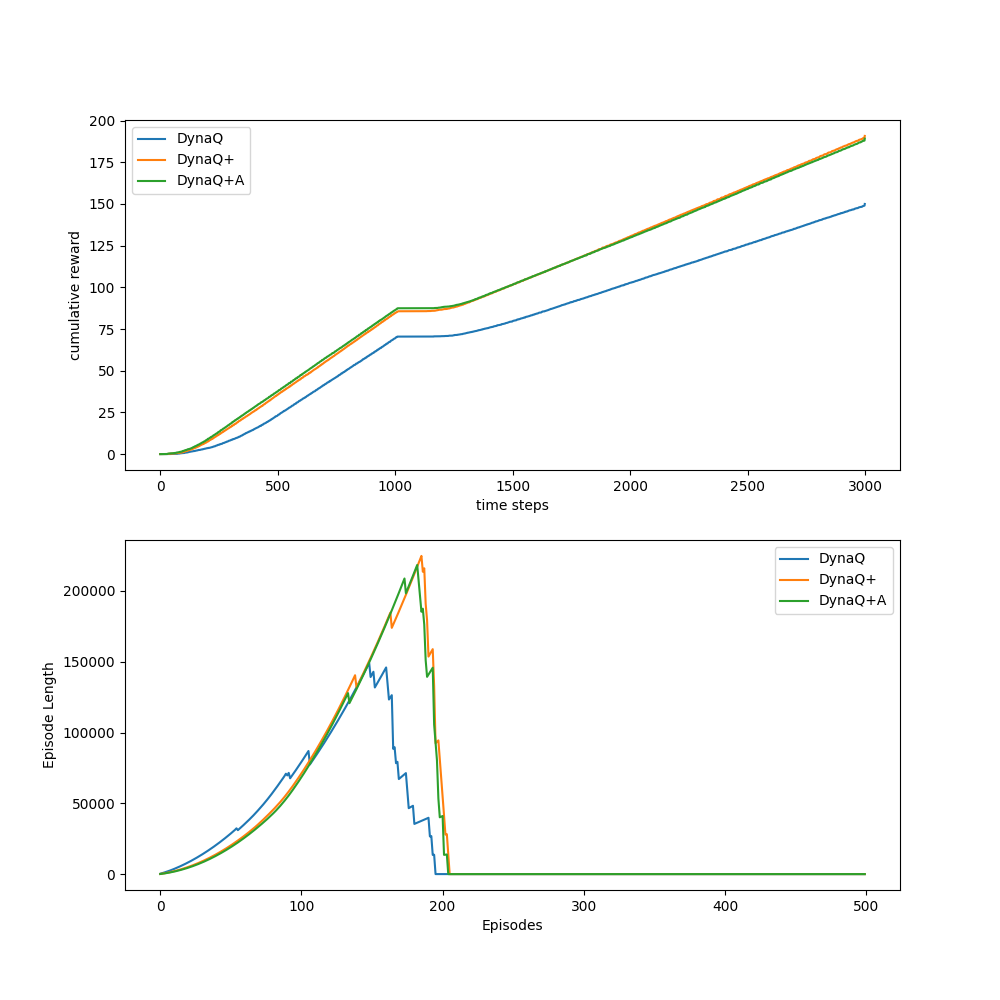
\includegraphics[scale=0.7]{example_8_4}

    Example 8.5 configuration.

    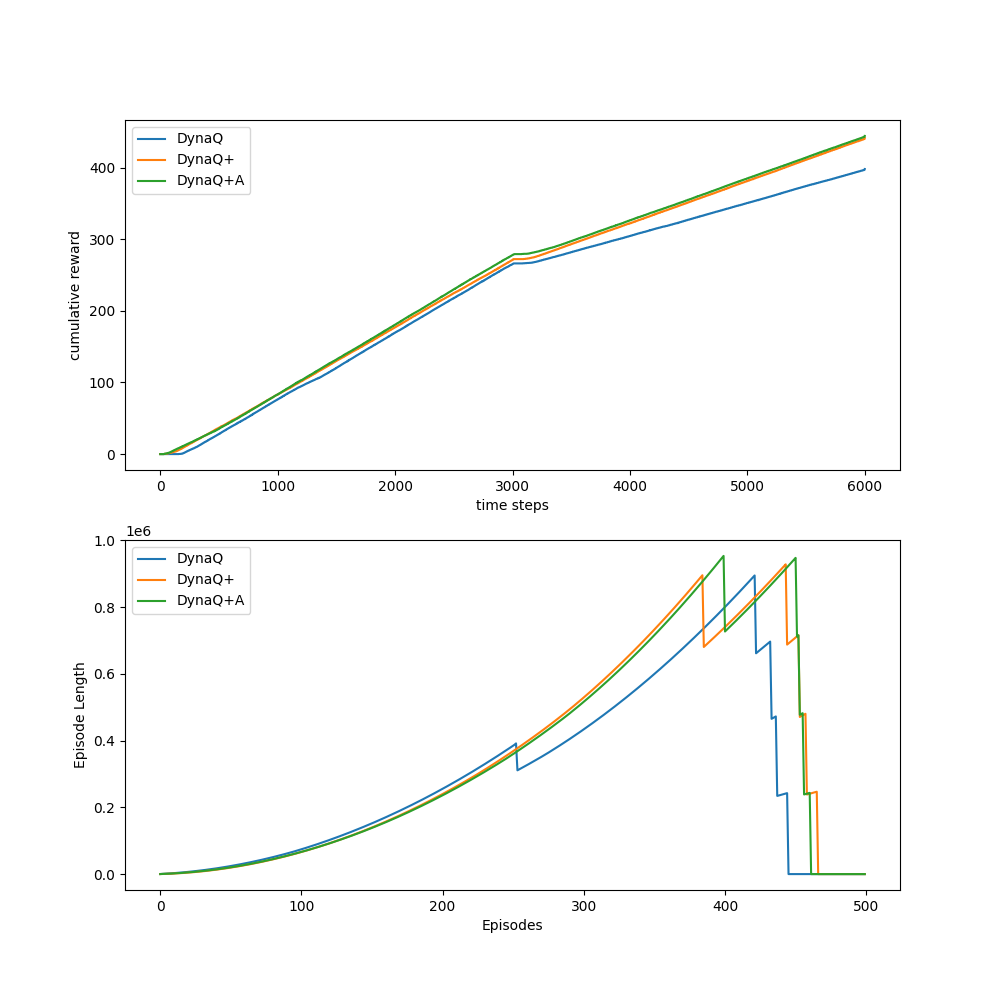
\includegraphics[scale=0.7]{example_8_4_2}

    The alternate DynaQ+ approach shows similar behaviour to that of DynaQ+.

    The alternate approach does not modify the q values.
    While the DynaQ+ approach encourage exploration of stages and new actions, the alternate approach only encourages exploring actions.
    Less calculation in planning phase may slightly reduce planning phase cost.

    \subsection{Question}

    How might the tabular Dyna-Q algorithm shown on page 164 be modified to handle stochastic environments?
    How might this modification perform poorly on changing environments such as considered in this section?

    How could the algorithm be modified to handle stochastic environments and changing environments?

    \subsection*{Answer}

    Deterministic algorithm keeps track of state action pairs and their q value.
    A stochastic algorithm should also keep track the number of times an action is taken and which next state is visited.
    Q value is formed as an expected value of possible next states and rewards.

    It may be necessary to apply expected value updates in planning as well.

    This approach is not suitable for changing environments.
    New transitions only will look like rare transitions to the algorithm.
    It will take a lot of time until new transitions gain significance.

    A solution would be to give more weight to recent transitions.


    \subsection{Question}

    The analysis above assumed that all of the b possible next states were equally likely to occur.
    Suppose instead that the distribution was highly skewed, that some of the b states were much more likely to occur than most.
    Would this strengthen or weaken the case for sample updates over expected updates?
    Support your answer.

    \subsection*{Answer}

    Highly skewed distributions strengthen the case for sample updates.

    With sampling high frequency states occur frequently and value function is updated accordingly.
    Value functions errors are reduced with very few updates.

    Expected updates on the other hand will waste effort on less likely states to decrease the error a little bit.


    \subsection{Question}

    Some of the graphs in Figure 8.8 seem to be scalloped in their early portions, particularly the upper graph for b = 1 and the uniform distribution.
    Why do you think this is?
    What aspects of the data shown support your hypothesis?

    \subsection*{Answer}

    In uniform case, start state is not updated as frequently.
    In on-policy case, the initial state is visited with a probability of 0.1 while the same probability is 1/states in uniform case.

    \subsection{Question}
    (programming) Replicate the experiment whose results are shown in the lower part of Figure 8.8, then try the same experiment but with b = 3.
    Discuss the meaning of your results.

    \subsection*{Answer}

    With 10.000 states, advantage of the on-policy approach is more obvious.

    When b=3, with 10.000 states, uniform approach can catch-up much later than it can do in 1000 states.

    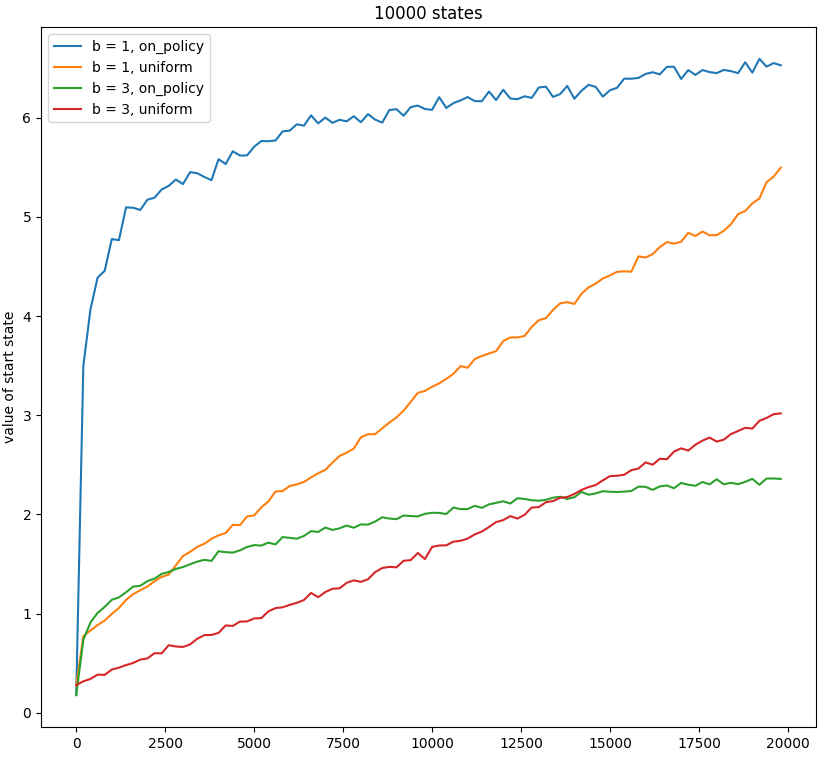
\includegraphics[scale=0.7]{exercise_8_8}



\end{document}


